\documentclass[11pt]{article}

% ------
% LAYOUT
% ------
\textwidth 165mm %
\textheight 230mm %
\oddsidemargin 0mm %
\evensidemargin 0mm %
\topmargin -15mm %
\parindent= 10mm

\usepackage[dvips]{graphicx}
\usepackage{multirow,multicol}
\usepackage[table]{xcolor}

\usepackage{amssymb}
\usepackage{amsfonts}
\usepackage{amsthm}

\graphicspath{{./pix/}} % put all your figures here.

\begin{document}
\begin{center}
\Large{\textbf{ECE 595: Homework 1}}

Your Name, Class ID

(Spring 2019)
\end{center}


\subsection*{Problem 1}
\noindent\textbf{General Principle}. Please type you solution in LaTeX. The margins should be approximately 1 inch on every side, and the font size should be no smaller than 11 point. The headline for every problem should be a \texttt{subsection} with no numbering.


\vspace{2ex}
\noindent\textbf{Collaboration}. If you collaborate with another student, you are still required to type your own solution. Please state at the header whom you have collaborated with. Two identical solutions without proper acknowledgement will be considered as plagiarism, and will be seriously penalized.




\vspace{2ex}
\noindent\textbf{Equations}. If you need to type an equation, make sure to only label the equations that will be referenced later. The standard notation for a scalar is $x \in \mathbb{R}$, a vector is $\mathbf{x} \in \mathbb{R}^n$, and a matrix is $\mathbf{A} \in \mathbb{R}^{m \times n}$. For example, the equation below shows a vector relationship between $\mathbf{x}$ and $\mathbf{y}$.
\begin{equation}
\mathbf{y} = \mathbf{A}\mathbf{x}.
\end{equation}


\vspace{2ex}
\noindent\textbf{Figure}. To insert a figure, you may use the command \texttt{includegraphics}. When inserting a figure, make sure that the resolution is high enough and the font of is readable. The general rule of thumb is that if you can read the figure at 100\% view (i.e., no zoom in), the figure is typically okay. When generating plots, please save them as \texttt{.pdf} or \texttt{.eps} because these are vectorized graphics files. We recommend you bold the curves so that they are more visible. Mark your axes and legends clearly. We reserve the right to not giving points to plots that are not readable.

\begin{figure}[h]
\centering
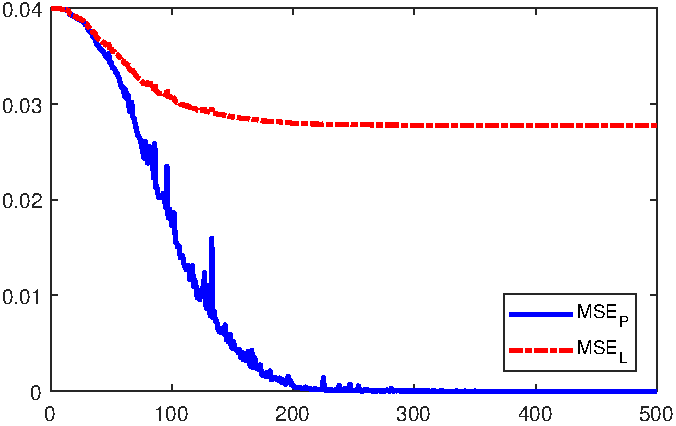
\includegraphics[width=0.5\linewidth]{MSE}
\caption{Example figure. Please type caption.}
\label{fig: figure 1}
\end{figure}




\subsection*{Problem 2}
Type your second problem here.


\subsection*{Problem 3}
Type your third problem here.











\end{document}

